\clearpage
\appendix

%\renewcommand\chaptername{Appendix}
%\renewcommand\thechapter{\arabic{chapter}}


%\renewcommand\chaptername{Appendix}            % hereafter, chapters are called "Appendix"
%\renewcommand\thechapter{\Alph{chapter}}       % chapter number in alph letters
%\renewcommand\thesection{\Alph{chapter}.\Roman{section}} % make sections "A.I"

%\renewcommand{\appendixname}{Appendix~\arabic{section}}

\setcounter{chapter}{0}
\setcounter{figure}{0}
\chapter{δ函数和傅里叶变换}	\label{A01}

% 更改公式标号格式
\counterwithout{equation}{chapter}		% 移除于chapter关联


% 正文

在这里我们不准备叙述$\delta$函数的严格数学理论,而只是将它作为一种方便的数学工具介绍给读者.

{\heiti 1. $\delta$函数的定义及基本性质}

以$f(x)$表示任何具有良好解析性质的函数.规定$\delta$函数的基本性质(也就是定义)为
\eqlong
\begin{empheq}{equation}\label{eqA1.1}
	\boxed{ \int_{a}^{b}f(x)\delta(x-x_{0})dx=f(x_{0}),\quad a<x_{0}<b
	}
\end{empheq}\eqnormal
显然,这定义等价于下列定义:
\begin{empheq}{align}\label{eqA1.2}
	&\int_{-\infty}^{\infty}f(x)\delta(x-x_{0})dx	\nonumber\\
	=&\int_{x_{0}-\varepsilon}^{x_{0}+\varepsilon}f(x)\delta(x-x_{0})dx=f(x_{0})
\end{empheq}
其中$\varepsilon$为任意小正数.通常,还可改用下列等价定义:
\begin{empheq}{equation}\label{eqA1.3}
	\begin{dcases}
		\delta(x-x_{0})=0,x\neq x_{0}	\\
		\int_{-\infty}^{\infty}\delta(x-x_{0})dx=1
	\end{dcases}
\end{empheq}\eqshort
容易证明,$\delta(x)$是偶函数,$\delta(x)=\delta(-x)$,并有性质
\begin{empheq}{equation}\label{eqA1.4}
	\delta(\lambda x)=\frac{1}{|\lambda|}\delta(x)
\end{empheq}
这公式在积分换元时很有用.

在\eqref{eqA1.1}式中取$f(x)=x-x_{0}$,则$f(x_{0})=0$,这结果适用于任何积分区间$(a,b)$,所以等价于
\begin{empheq}{equation}\label{eqA1.5}
	(x-x_{0})\delta(x-x_{0})=0
\end{empheq}\eqllong


{\heiti 2. $\delta$函数的具体表示}

某些含参数的函数,当参数趋于某种极限时,就成为$\delta$函数.最常用的有下列几种
\begin{empheq}{equation}\label{eqA1.6}
(\ce{i})\qquad\qquad\qquad \delta(x)=\lim\limits_{\alpha\rightarrow0}\frac{1}{\sqrt{\pi}\alpha}e^{-x^{2}/\alpha}
\end{empheq}
这个函数符合定义\eqref{eqA1.3}式,其图形如附录图1所示,曲线下面的面积为1,有效宽度大致为$2\alpha$.
\begin{empheq}{equation}\label{eqA1.7}
(\ce{ii})\qquad\qquad\qquad \boxed{\delta(x)=\lim_{\alpha\rightarrow\infty}\frac{\sin\alpha x}{\pi x} }
\end{empheq}\eqnormal
其图形如附录图2所示,为振荡衰减型,有效宽度大致为$\frac{2\pi}{\alpha}$.在$|x|>\frac{\pi}{\alpha}$区域,由于迅速振荡,对积分无贡献.而全空间积分等于1:
\begin{empheq}{equation*}
	\int_{-\infty}^{\infty}\frac{\sin\alpha x}{\pi x}dx=\frac{1}{\pi}\int_{-\infty}^{\infty}\frac{\sin t}{t}dt=1.
\end{empheq}\eqllong
\begin{figure}[!h]
	\centering
	\small
	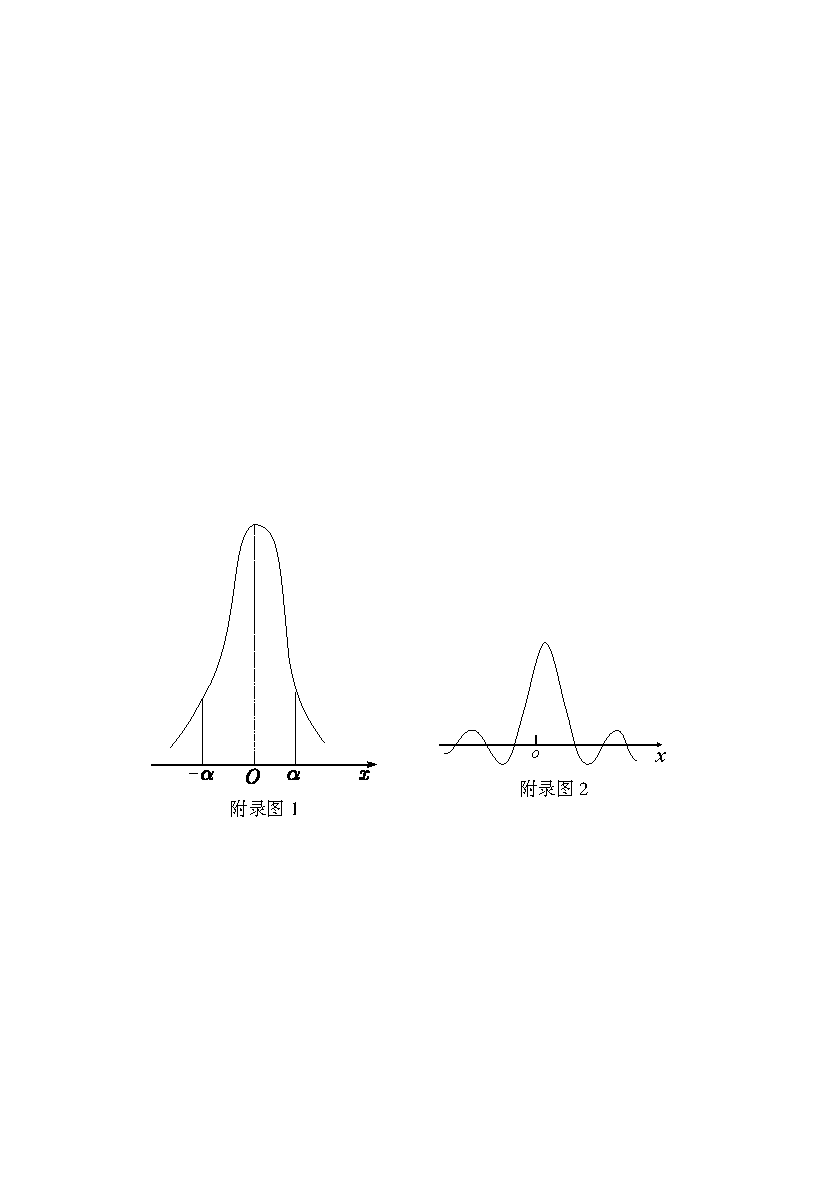
\includegraphics[width=8cm,clip]{QM file/figure/A-1,2}
	\caption*{}\label{fig.A-1,2}
\end{figure}
\begin{empheq}{equation}\label{eqA1.8}
(\ce{iii})\qquad\qquad\qquad \boxed{\delta(x)=\frac{1}{2\pi}\int_{-\infty}^{\infty}e^{ikx}dk }
\end{empheq}\eqnormal
由于$e^{ikx}=\cos kx+i\sin kx$,如将\eqref{eqA1.8}式中积分上下限改写为$\pm\alpha(\alpha\rightarrow\infty)$,立即可以发现\eqref{eqA1.8}式与\eqref{eqA1.7}式是等价的.

{\heiti 3. 傅里叶变换}

将任何具有良好解析性质的函数$f(x)$表示成傅里叶积分的形式
\begin{empheq}{equation}\label{eqA1.9}
	f(x)=\frac{1}{\sqrt{2}}\int_{-\infty}^{\infty}g(k)e^{ikx}dk
\end{empheq}\eqlllong
$g(k)$称为$f(x)$的傅里叶变换式.利用$\delta$函数很容易导出$g(k)$的公式,如下.利用\eqref{eqA1.8}式,将$f(x)$表示成
\begin{empheq}{align*}
	f(x)&=\int_{-\infty}^{\infty}f(x^{\prime})\delta(x-x^{\prime})dx^{\prime}
	&=\frac{1}{2\pi}\iint_{-\infty}^{\infty}f(x^{\prime})e^{ik(x-x^{\prime})}dkdx^{\prime}
\end{empheq}\eqnormal
与\eqref{eqA1.9}式比较,即得
\begin{empheq}{align}\label{eqA1.10}
	g(k)&=\frac{1}{\sqrt{2}}\int_{-\infty}^{\infty}f(x^{\prime})e^{-ikx^{\prime}}dx^{\prime}	\nonumber\\
	&=\frac{1}{\sqrt{2}}\int_{-\infty}^{\infty}f(x)e^{-ikx}dx
\end{empheq}
此即傅里叶变换式.注意\eqref{eqA1.9}、\eqref{eqA1.10}式结构的对称性.

{\heiti 4. 三维情形}

三维$\delta$函数定义为
\begin{empheq}{equation}\label{eqA1.11}
	\delta(\boldsymbol{r}-\boldsymbol{r}_{0})=\delta(x-x_{0})\delta(y-y_{0})\delta(z-z_{0})
\end{empheq}
其中
\begin{empheq}{equation*}
	\boldsymbol{r}=(x,y,z),\quad \boldsymbol{r}_{0}=(x_{0},y_{0},z_{0})
\end{empheq}
基本积分性质为
\begin{empheq}{equation}\label{eqA1.12}
	\boxed{ \iiint_{-\infty}^{\infty}f(\boldsymbol{r})\delta(\boldsymbol{r}-\boldsymbol{r}_{0})d^{3}\boldsymbol{r}=f(\boldsymbol{r}_{0})
	}
\end{empheq}
与\eqref{eqA1.4}式相应,有关系
\begin{empheq}{equation}\label{eqA1.13}
	\delta(\lambda\boldsymbol{r}-\lambda\boldsymbol{r}_{0})=\frac{1}{|\lambda^{3}|}\delta(\boldsymbol{r}-\boldsymbol{r}_{0})
\end{empheq}
\eqref{eqA1.8}式推广成
\begin{empheq}{equation}\label{eqA1.14}
	\delta(\boldsymbol{r})=\frac{1}{(2\pi)^{3}}\iiint_{-\infty}^{\infty}e^{i\boldsymbol{k}\cdot\boldsymbol{r}}d^{3}\boldsymbol{k}
\end{empheq}
利用此式容易导出三维傅里叶变换公式
\begin{empheq}{equation}\label{eqA1.15}
	\boxed{\begin{aligned}
		f(\boldsymbol{r})=\left(\frac{1}{2\pi}\right)^{\frac{3}{2}}\iiint_{-\infty}^{\infty}g(\boldsymbol{k})e^{i\boldsymbol{k}\cdot\boldsymbol{r}}d^{3}\boldsymbol{k}	\\
		g(\boldsymbol{k})=\left(\frac{1}{2\pi}\right)^{\frac{3}{2}}\iiint_{-\infty}^{\infty}f(\boldsymbol{r})e^{i\boldsymbol{k}\cdot\boldsymbol{r}}d^{3}\boldsymbol{r}
	\end{aligned}}
\end{empheq}

采用球坐标$(r,\theta,\varphi)$时,当$r\rightarrow0$,角$\theta,\varphi$失去意义,这时常用径向$\delta$函数$\delta(r)$代替$\delta(\boldsymbol{r})$.考虑到$r$的变化范围是$0\leqslant r<\infty$,$\delta$函数是偶函数,以及$d^{3}\boldsymbol{r}\Rightarrow r^{2}drd\Omega$,
\begin{empheq}{align*}
	 &\iiint_{-\infty}^{\infty}\delta(\boldsymbol{r})d^{3}\boldsymbol{r}=1=2\int_{0}^{\infty}\delta(r)dr	\\
	=&\frac{1}{2\pi}\int d\Omega\int_{0}^{\infty}\frac{\delta(r)}{r^{2}}r^{2}dr	\\
	=&\frac{1}{2\pi}\iiint_{-\infty}^{\infty}\frac{\delta(r)}{r^{2}}d^{3}\boldsymbol{r}
\end{empheq}\eqshort
因此
\begin{empheq}{equation}\label{eqA1.16}
	\delta(\boldsymbol{r})=\frac{1}{2\pi r^{2}}\delta(r)
\end{empheq}\eqnormal
注意
\begin{empheq}{equation}\label{eqA1.17}
	\int_{-\infty}^{\infty}f(r)\delta(r)dr=\frac{1}{2}f(0)
\end{empheq}

